\documentclass{article}
\usepackage{tikz}
\usetikzlibrary{automata,positioning}

\begin{document}

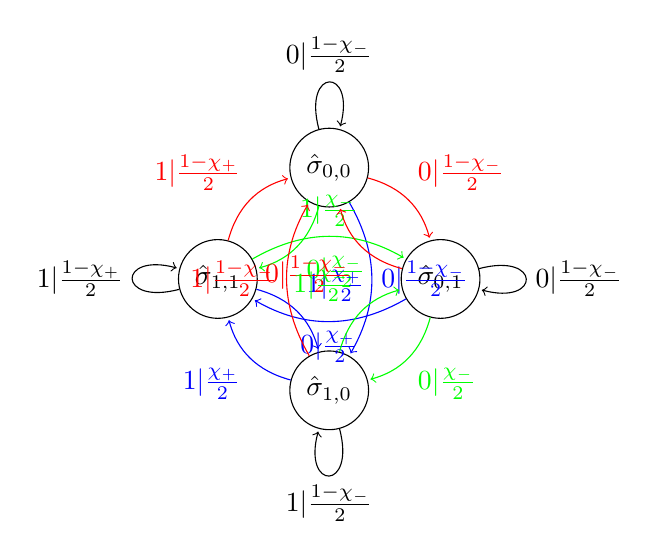
\begin{tikzpicture}[shorten >=1pt,node distance=2cm,on grid,auto]
    \node[state] (q_0) {$\hat{\sigma}_{0,0}$};
    \node[state] (q_1) [below left of=q_0] {$\hat{\sigma}_{1,1}$};
    \node[state] (q_2) [below right of=q_0] {$\hat{\sigma}_{0,1}$};
    \node[state] (q_3) [below right of=q_1] {$\hat{\sigma}_{1,0}$};

    \path[->]
        (q_0) edge [loop above] node {$0|\frac{1-\chi_-}{2}$} ()
              edge [bend left,red] node {$0|\frac{1-\chi_-}{2}$} (q_2)
              edge [bend left,blue] node {$0|\frac{1-\chi_-}{2}$} (q_3)
              edge [bend left,green] node {$0|\frac{\chi_-}{2}$} (q_1)
        (q_1) edge [loop left] node {$1|\frac{1-\chi_+}{2}$} ()
              edge [bend left,red] node {$1|\frac{1-\chi_+}{2}$} (q_0)
              edge [bend left,blue] node {$1|\frac{\chi_+}{2}$} (q_3)
              edge [bend left,green] node {$1|\frac{\chi_-}{2}$} (q_2)
        (q_2) edge [loop right] node {$0|\frac{1-\chi_-}{2}$} ()
              edge [bend left,red] node {$0|\frac{1-\chi_-}{2}$} (q_0)
              edge [bend left,blue] node {$0|\frac{\chi_+}{2}$} (q_1)
              edge [bend left,green] node {$0|\frac{\chi_-}{2}$} (q_3)
        (q_3) edge [loop below] node {$1|\frac{1-\chi_-}{2}$} ()
              edge [bend left,red] node {$1|\frac{1-\chi_-}{2}$} (q_0)
              edge [bend left,blue] node {$1|\frac{\chi_+}{2}$} (q_1)
              edge [bend left,green] node {$1|\frac{\chi_-}{2}$} (q_2);
\end{tikzpicture}

\end{document}